\subsection{Impedancia de entrada}

En los siguientes gr\'aficos se observa la impedancia de entrada medida y simulada con el m\'etodo de Montecarlo.
\begin{figure}[H] %!ht
	\centering
	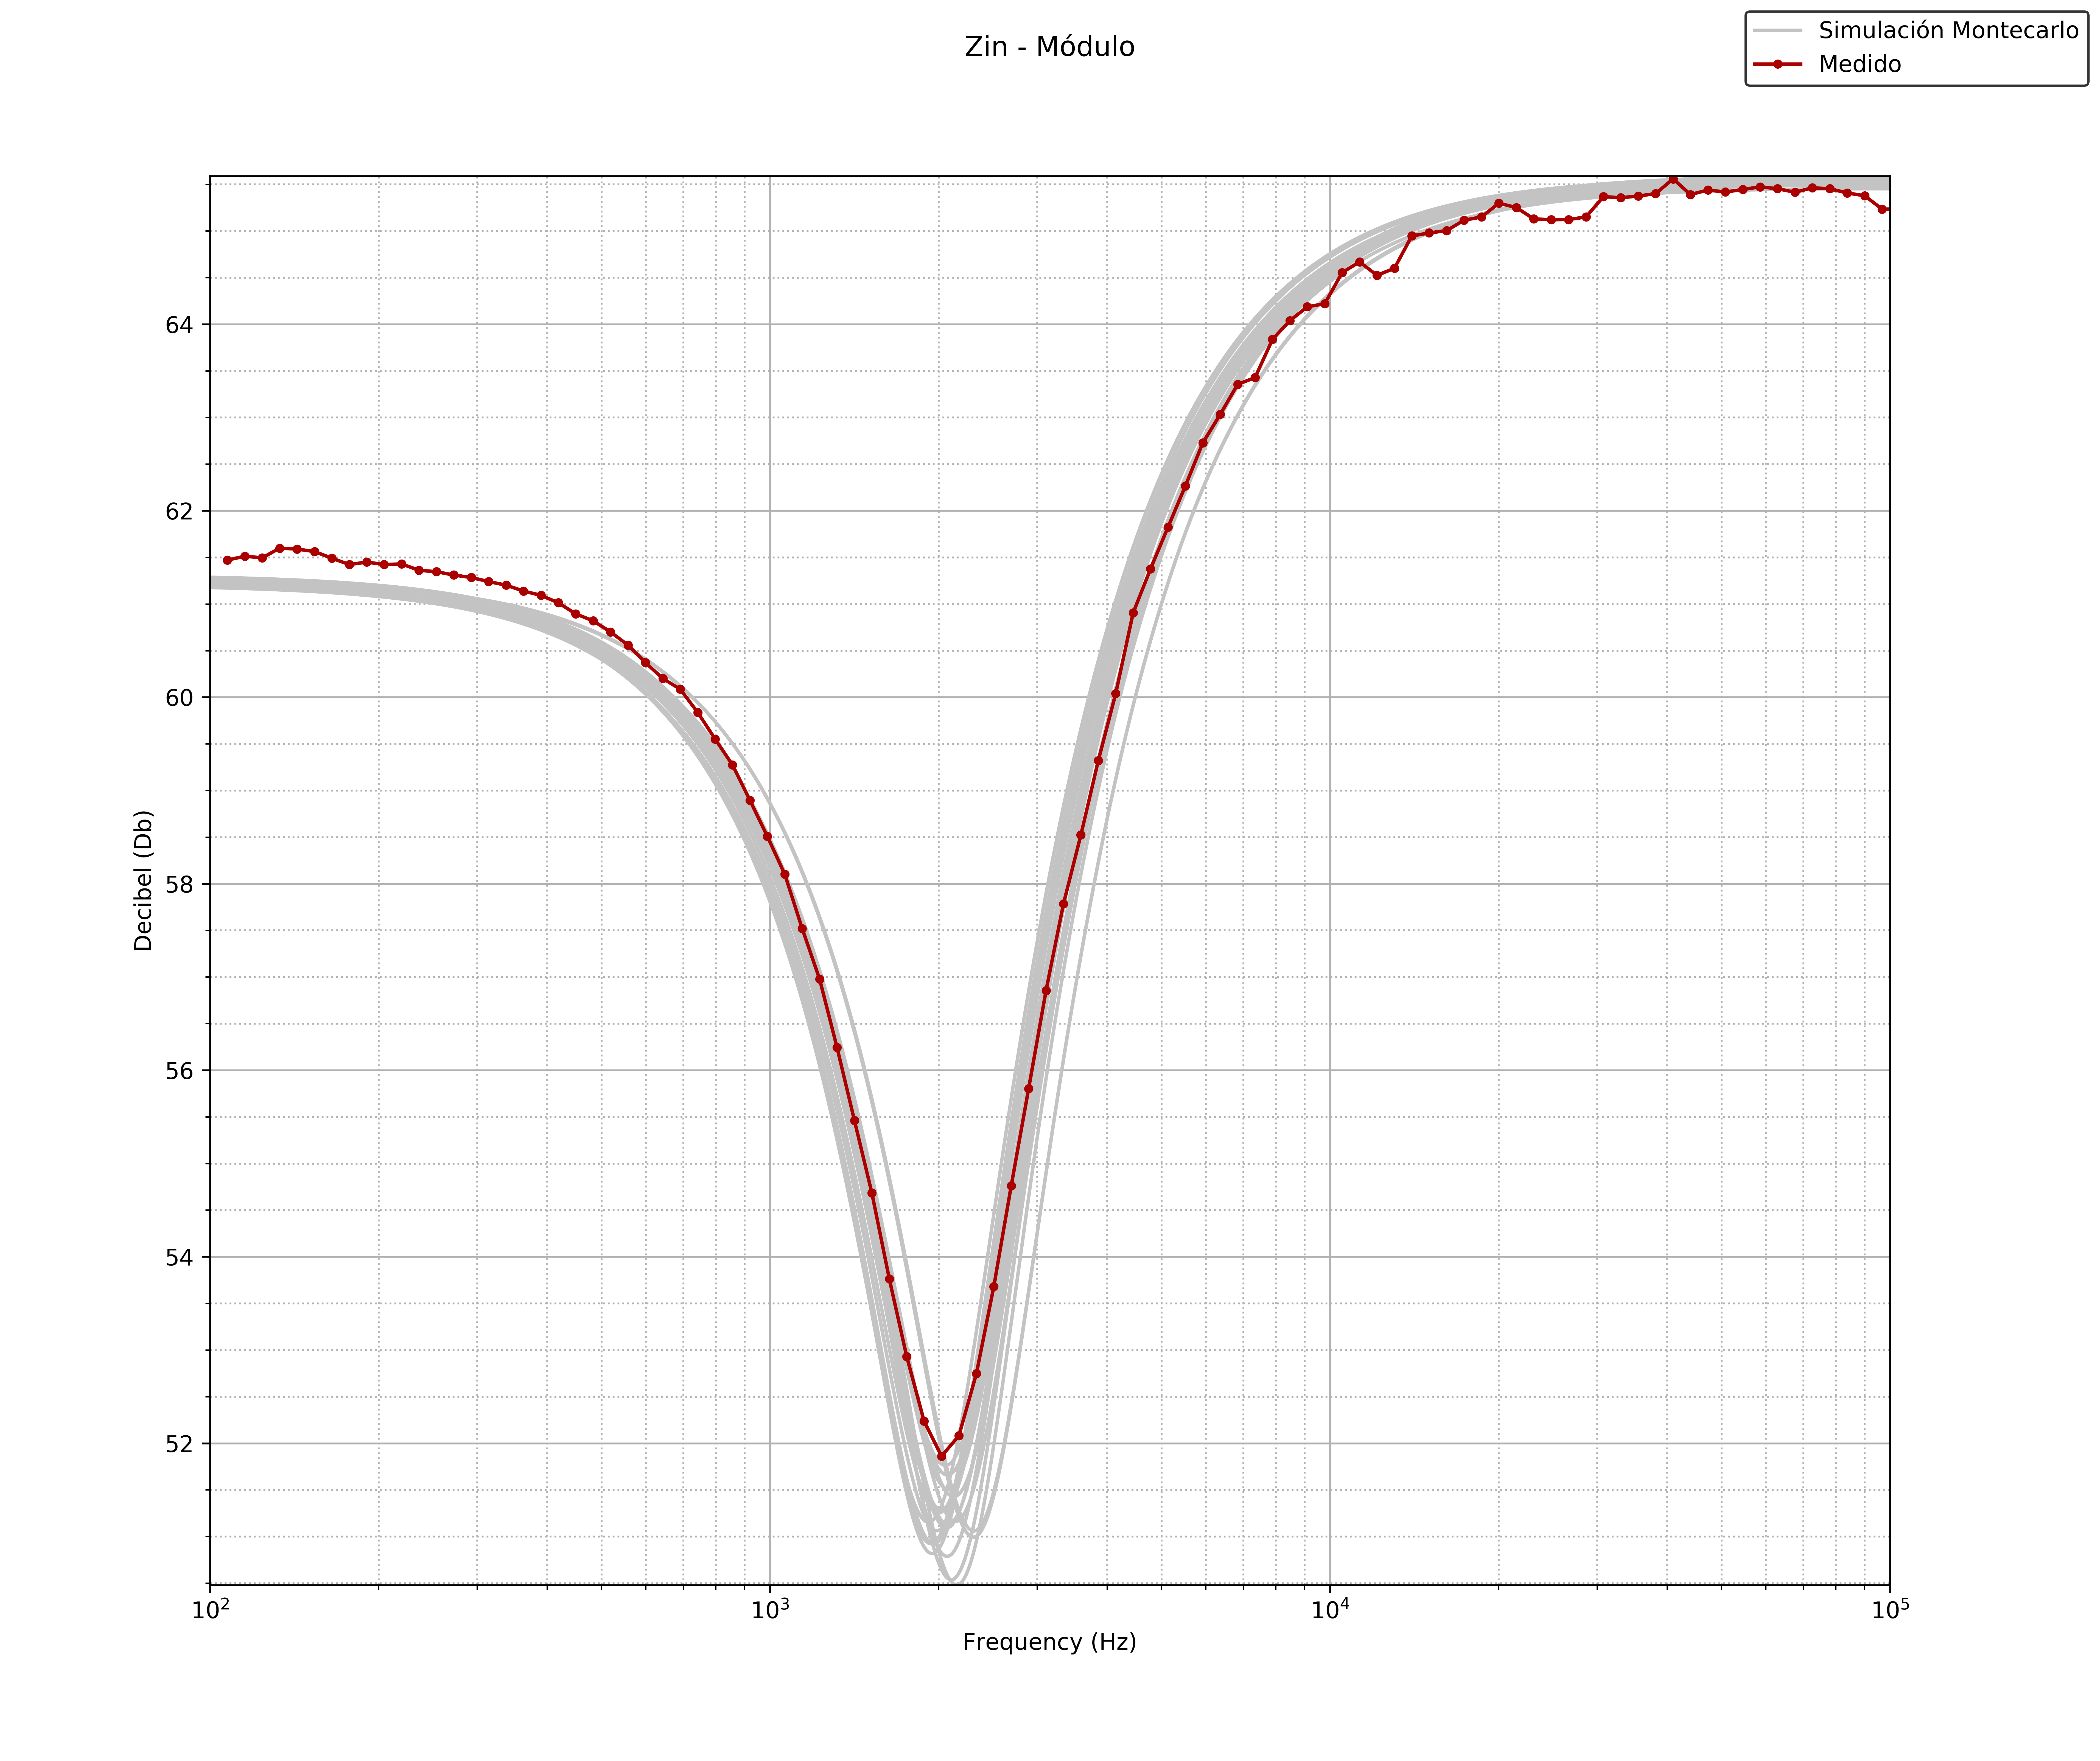
\includegraphics[width=10cm,height=10cm,keepaspectratio]{../EJ1/00GRAFICOS/zin_modulo_sinTeorico.png}
	\caption{Impedancia de entrada.}
	\label{zin_mod}
\end{figure}

\subsection{Impedancia de salida}

En esta parte se detallar\'a el m\'etodo empleado para medir la impedancia de salida, pero se anticipa al lector que no se considera que el mismo haya funcionado como se esperaba.
\begin{figure}[H] %!ht
	\centering
	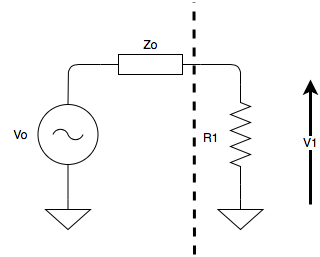
\includegraphics[width=8cm,height=8cm,keepaspectratio]{../EJ1/00GRAFICOS/zout.png}
	\caption{Impedancia de entrada.}
	\label{zout}
\end{figure}